\chapter{Architektur und Implementierung des Textsatzsystems}\label{ch-architektur}

In diesem Kapitel wird der architekturelle Aufbau des Anwendungsfalls
„Textsatzsystem“ beschrieben.

Dazu gehört zum einen die Zielarchitektur,
welche zur Darstellung des resultierenden Dokuments dient, beschrieben in
Kapitel \ref{sec-zielarchitektur}.

Zum anderen wird in Kapitel \ref{sec-scalaDSL} die DSL beschrieben,
welche eine wohlgeformte Schnittstelle für den Benutzer darstellt,
sowie diverse Automatisierungsfähigkeiten übernimmt, wie z.B.
die Durchnummerierung von Kapiteln.

\section{Zielarchitektur}\label{sec-zielarchitektur}

Wie in Kapitel \ref{sec-zielarchitektur} schon beschrieben wurde, ist die
Zielarchitektur für die Darstellung des Dokuments verantwortlich, welche
auf Webtechnologie basiert und somit von einem Webbrowser gerendert wird.

Da Webtechnologie, insbesondere HTML/CSS, keine Möglichkeiten bietet
Seiten wie z.B. im DIN A4 Format darzustellen ist \emph{die}
Hauptaufgaben eine geeignete \emph{Abstraktion für Seiten} zu entwickeln.
Eine detaillierte Beschreibung ist in Kapitel \ref{sec-abstrationSeiten}.

Weiterhin ist wichtig, wie die einzelnen Entitäten, wie Überschriften,
Texte, Bilder etc. erstellt werden können---dies soll in Kapitel
\ref{sec-templating} geklärt werden.

Eine Übersicht über die Anforderungen ist in Kapitel
\ref{sec-ziel_anforderungen} aufgelistet.

Der komplette Quellcode mit Tests und weiteren Beispielen ist im
Github Repositorium unter \url{https://github.com/themerius/ScalTeX-templates}
zu finden.

\subsection{Anforderungen}\label{sec-ziel_anforderungen}

Das kleine JavaScript-Framework wird mit dem
\emph{behavior-driven development}\footnote{
Alternative bzw. Weiterentwicklung des test-driven development.
\url{http://dannorth.net/introducing-bdd/}.}
Paradigma entwickelt, für diesen Zweck kommt das
Jasmine-Framework\footnote{\url{http://pivotal.github.com/jasmine/}}
zum Einsatz.

\emph{Anmerkung:}
Die Spezifikationen sind in englischer Sprache verfasst, da dies die
Verkehrssprache der Informatik darstellt und es guter Stil ist, wenn der
Programmcode konsequent auf englischsprachige Dokumentation setzt.

\begin{itemize}
  \item Util
    \begin{itemize}
      \item should determine the dpi used by the browser
      \item should calculate the browser specific `pixels per mm`
      \item should be a singleton
      \item should be able to transform mm to px
    \end{itemize}
  \item Entity (siehe Kapitel \ref{sec-templating})
    \begin{itemize}
      \item should create an element out of template and json
      \item should be able to append the created element to another
            element with an id
      \item should know it's actual height
      \item should be able to modify or extend the json
    \end{itemize}
  \item Page (siehe Kapitel \ref{sec-abstrationSeiten})
    \begin{itemize}
      \item should know the type and id for every configured append point
      \item should know it's maximum height for every append point
      \item should create a new element out of a page template and
            configured append points
      \item should be append-able to another element with an id
      \item should know the available space on the page resp. it's
            append points
    \end{itemize}
  \item PageFactory (siehe Kapitel \ref{sec-abstrationSeiten})
    \begin{itemize}
      \item should save the (maybe incomplete) page configurations
            with a related name
      \item should combine the page configs with other page config fragments
            to a complete page config
      \item should produce Page instances out of a certain page config and
            other page config fragments
    \end{itemize}
  \item Areal (siehe Kapitel \ref{sec-areal})
    \begin{itemize}
      \item should be able prepare a construction area for every page type
      \item should generate entities out of a json-sequence and keep them
      \item should generate the special entities, which are individual
            for every page
      \item should mount the entities into the targeted construction area
      \item should create new pages for viewing, with footer, and move the
            entities to fill the pages
      \item should keep track of the page numbers of the viewed pages
      \item should be able to destruct the construction areas
    \end{itemize}
\end{itemize}

\subsection{Abstraktion für Seiten}\label{sec-abstrationSeiten}

Um eine solche Abstraktion zu ermöglichen wird die Hilfe von JavaScript
benötigt, welches dafür sorgt, dass das Dokument an den richtigen Stelle auf
entsprechende Seiten umgebrochen wird.

\paragraph{Vorarbeit}
Zunächst muss mit gewöhnlichem HTML plus CSS eine „Webseite“ angefertigt
werden, die den Inhalt in eine z.B. DIN A4 Seite hüllt. Diese Konstruktion
kann später von dem JavaScript-Framework vervielfältigt und mit entsprechendem
Inhalt gefüllt werden. Wie es beispielhaft auf auf Abbildung
\ref{fig-one_page} zu sehen ist,
kann man gut die Seite mit ihren inneren und äußeren
Grenzen erkennen. Wenn jetzt weitere Texte und Bilder
hinzukommen, wächst der Inhalt über die Seite hinaus. Wir brauchen nun
eine Strategie, um dies zu vermeiden und neue Seiten einzufügen, auf denen
der Inhalt fortgesetzt werden kann.

\newpage
\begin{figure}[h!]
  \centering
    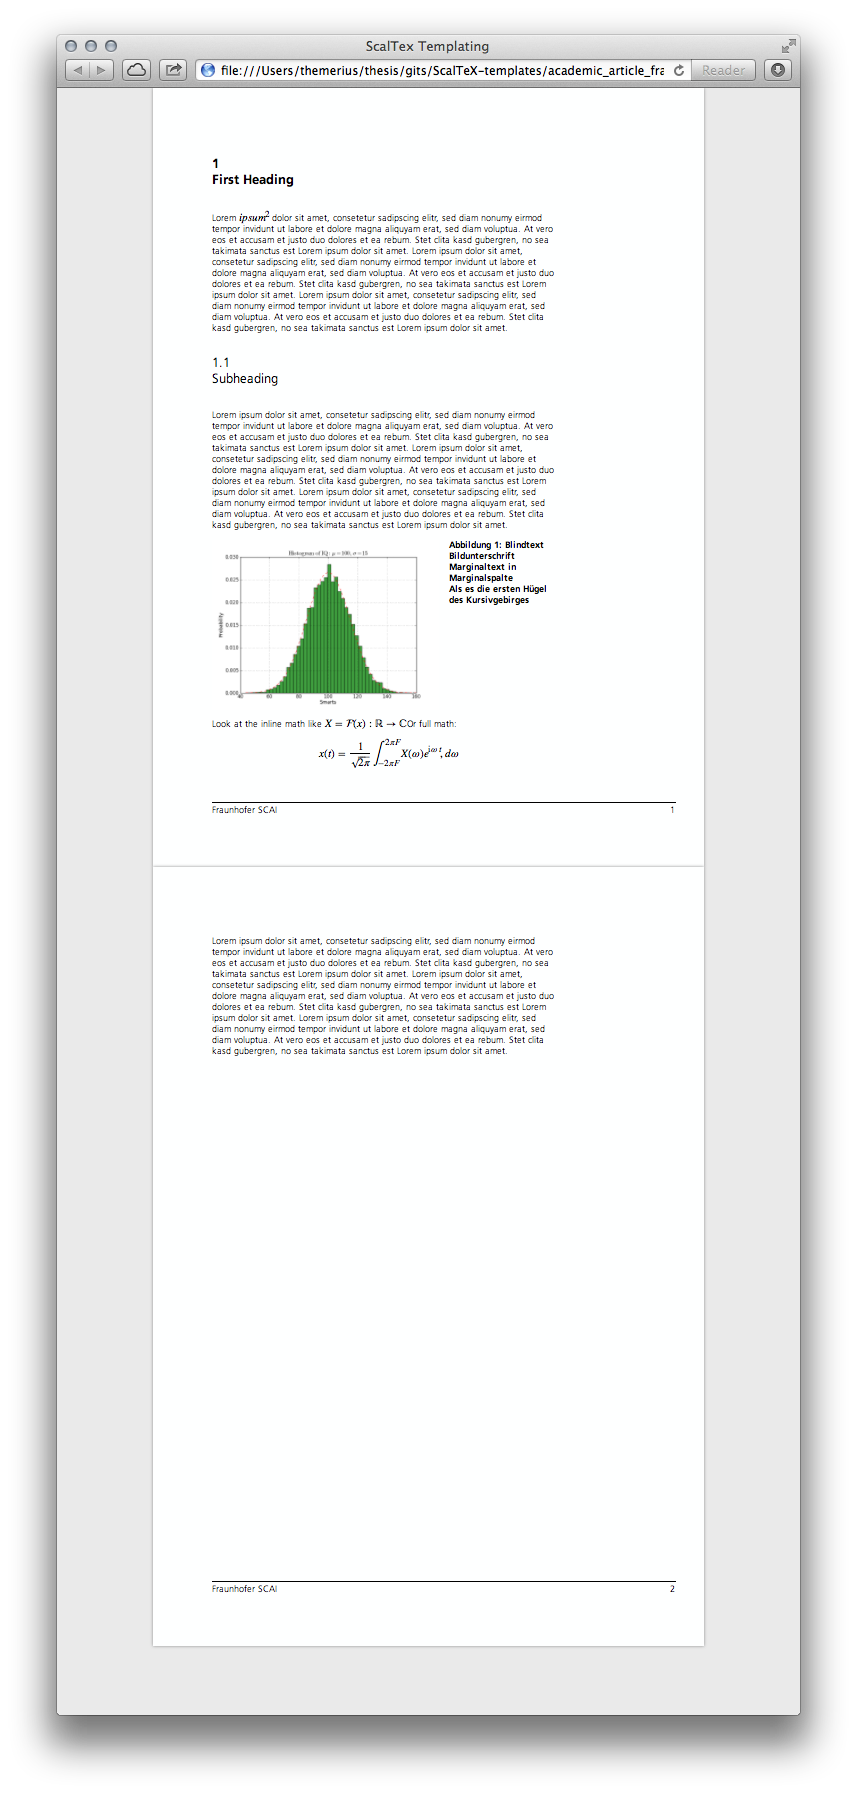
\includegraphics[height=0.9\textheight]{figures/two_pages.png}
  \caption{Zwei DIN A4 Seiten mit HTML und CSS gesetzt im Fraunhofer Corporate Design.}\label{fig-one_page}
\end{figure}
\newpage

\paragraph{Strategie}
Diese konzentriert sich zunächst darauf die Entitäten, wie Texte, Bilder usw.,
auf Seiten entsprechend dem Dokumentenfluss zuzuweisen.
In diesem Fall darf zunächst eine
einzelne Entität nicht die Größe einer Seite überschreiten---diese
Problematik soll später näher erläutert werden.

Der prinzipielle Ablauf wird auf Abbildung \ref{fig-aufteilungsstrategie}
visualisiert. Rechts ist die temporäre \emph{Construction Page}, die zum
ausmessen der Entitäten dient. Für jeden Seitentypus welcher vom jeweilige
Dokumenten-Template angeboten wird gibt es also eine Construction Page, sofern
dieser sich von den Ausmaßen anderes verhalten sollte.

Der Ablauf ist also wie folgt: die Entität wird mithilfe der Construction
Page ausgemessen und wenn auf der \emph{View Page} noch genügend Platz
vorhanden ist dort hin verschoben, wenn nicht genügend Platz vorhanden ist,
wird eine neue Seite erstellt und die Entität dort platziert.

Hier kann noch ein Zwischenschritt eingefügt werden, der es ermöglichen
sollte, gerade Textentitäten, weiter aufteilen zu können, so dass eine
bessere Auslastung der Seiten erreicht werden kann.

\newpage
\begin{figure}[h!]
  \centering
    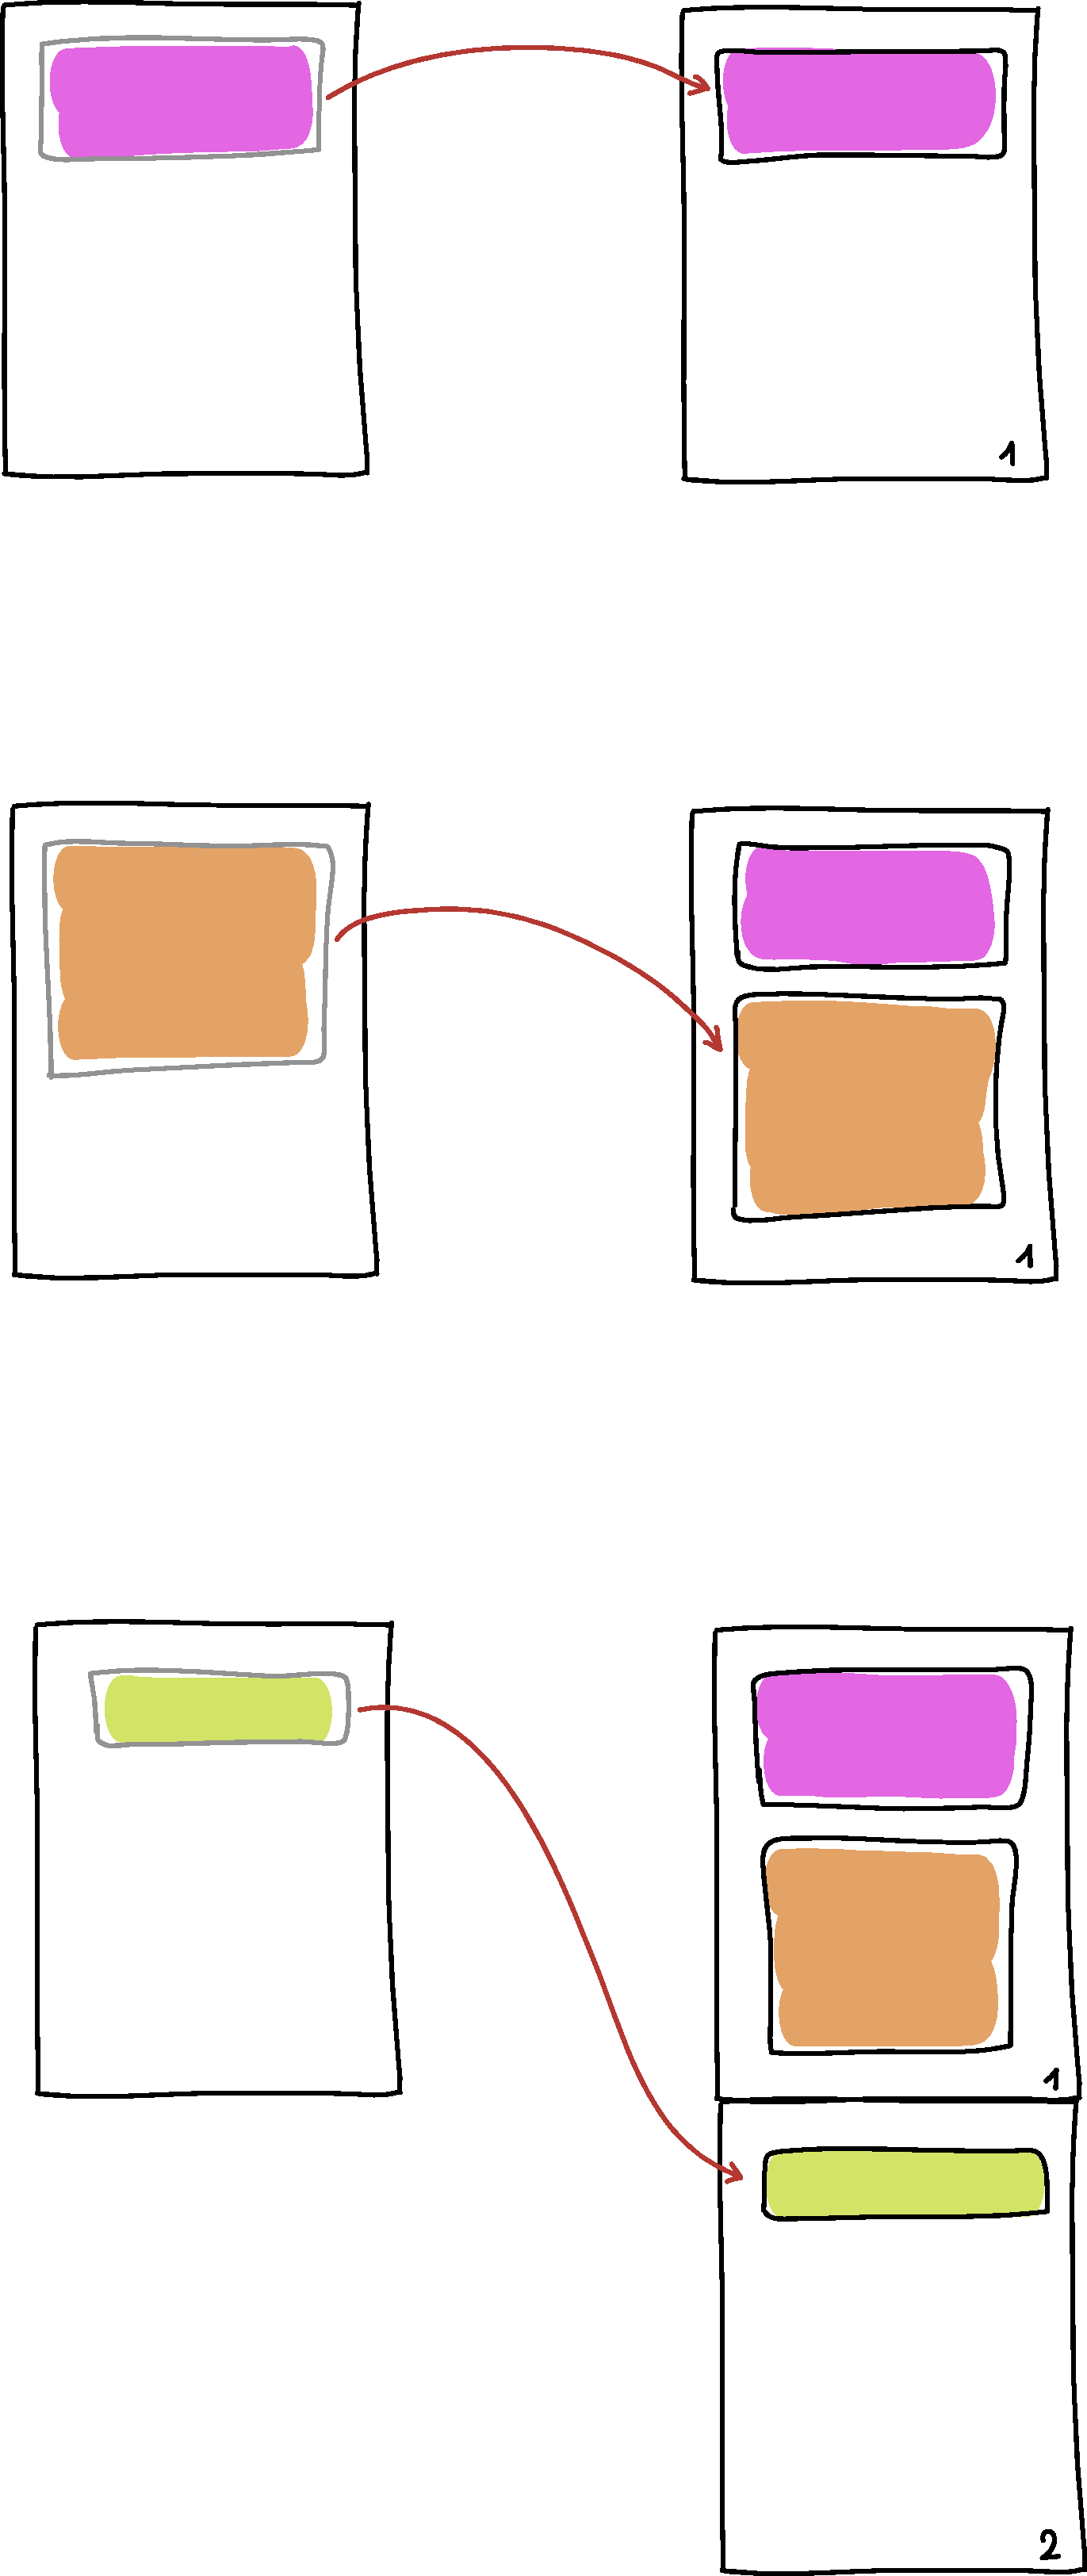
\includegraphics[height=0.9\textheight]{figures/aufteilungsstrategie.pdf}
  \caption{Aufteilungsstrategie, wie Entitäten auf einzelne Seiten
           verteilt werden. Rechts ist die \emph{Construction Page},
           links sind die \emph{View Pages}.}
  \label{fig-aufteilungsstrategie}
\end{figure}
\newpage

\subsection{Templating}\label{sec-templating}

Ich habe mich dazu entschieden das Templating vorerst mit JavaScript
vorzunehmen, also komplett auf der Seite des Dokumenten-Betrachters.
Dies soll den Zweck haben, dass ein Dokumenten-Template-Designer es
leichter haben soll sein Dokumenten-Design zu bauen und zu debuggen --
komplett unabhängig von der DSL bzw. der Programmierlogik.
Zum Einsatz kommt dabei die Javascript-Bib\-lio\-thek
\emph{mustache}\footnote{\url{http://mustache.github.com}}.

Auf diese Weise kann jede einzelne Entität oder Seite clientseitig
durch ein kleines Template-Snippet darstellt werden, welches an die
Bedürfnisse des spezifischen Dokumenten-Designs bzw. Dokumenten-Templates
angepasst ist. Beispielsweise eine Überschrift, könnte so aussehen:

\begin{verbatim}
<script id="heading" type="text/template">
<div class="row">
  <div class="col4">
    <{{h}}>{{number}}
      </br>
      {{heading}}
    </{{h}}>
    </br></br>
  </div>
  <div class="row-end">&nbsp;</div>
</div>
</script>
\end{verbatim}

Diese muss dann nur noch von der DSL entsprechend mit einer
JSON-Daten\-struktur\footnote{JSON ist die \emph{JavaScript Object Notation},
und bildet die zentrale Datenstruktur von JavaScript.
Mehr Informationen unter \url{http://json.org}.} gefüttert werden bzw.
instanziiert werden, wie z.B.:

\begin{verbatim}
{
  heading: "First Heading",
  number: 1,
  h: "h1"
};
\end{verbatim}

\subsection{Dokumenten-Areale}\label{sec-areal}

Die resultierenden Seiten zur Anzeige (View Pages), werden bestimmten
Arealen zugeordnet, diese dienen insbesondere der logischen Strukturierung
des Dokuments. Aus Sicht der Seiten sind diese Areale quasi
Einhängepunkte, wo die fertig gefüllten Seiten angefügt werden.

Innerhalb des HTML-Dokuments können diese Areale in ihrer Reihenfolge
verändert werden, und ermöglichen so einen recht flexiblen Umgang mit
den Doku\-men\-ten-Arealen.

\begin{verbatim}
<div id="TitlepageAreal"></div>
<div id="TableOfContentsAreal"></div>
<div id="DocumentAreal"></div>
\end{verbatim}

Es muss nur dem JavaScript-Framework welches die Abstraktion für die
Seiten vornimmt mitgeteilt werden, für welche IDs, welche Areale definiert
sind.

\subsection{Aufbau HTML-Datei}\label{sec-html-datei}

Der prinzipielle Aufbau bzw. Reihenfolge einer fertigen HTML-Datei
mit allen benötigen Elementen der Zielarchitektur ist in Abbildung
\ref{fig-zielarchitektur_aufbau} illustriert. Komplette Beispiele
sind im git-Repositorum zu finden. Im \emph{Header} sind die üblichen
HTML-Header-Deklarationen, wie z.B. die Einbindung von CSS-Dateien. Mit den
\emph{Areal Append Points} sind jene aus Kapitel \ref{sec-areal}
gemeint. Gefolgt von \emph{Entity Templates} und deren \emph{Instanzen},
in Form von JSON-Repräsentationen, wie in Kapitel \ref{sec-templating}
beschrieben. Danach werden die \emph{Special Entities} erzeugt, was z.B.
eine Fußzeile sein kann, welche nur einmal konfiguriert werden muss,
da sie auf jeder Seite quasi gleich ist, bis auf bsplw. die Seitennummer.
Die \emph{Page Factory}, welche neue Seiten produzieren kann, muss noch
konfiguriert werden, danach folgt das \emph{Areal Setup} wo alle Informationen
zusammenlaufen und wo auch das entgültige Dokument gesetzt wird.
Der \emph{Footer} schließt lediglich alle HTML-Tags.

\begin{figure}[h!]
  \centering
    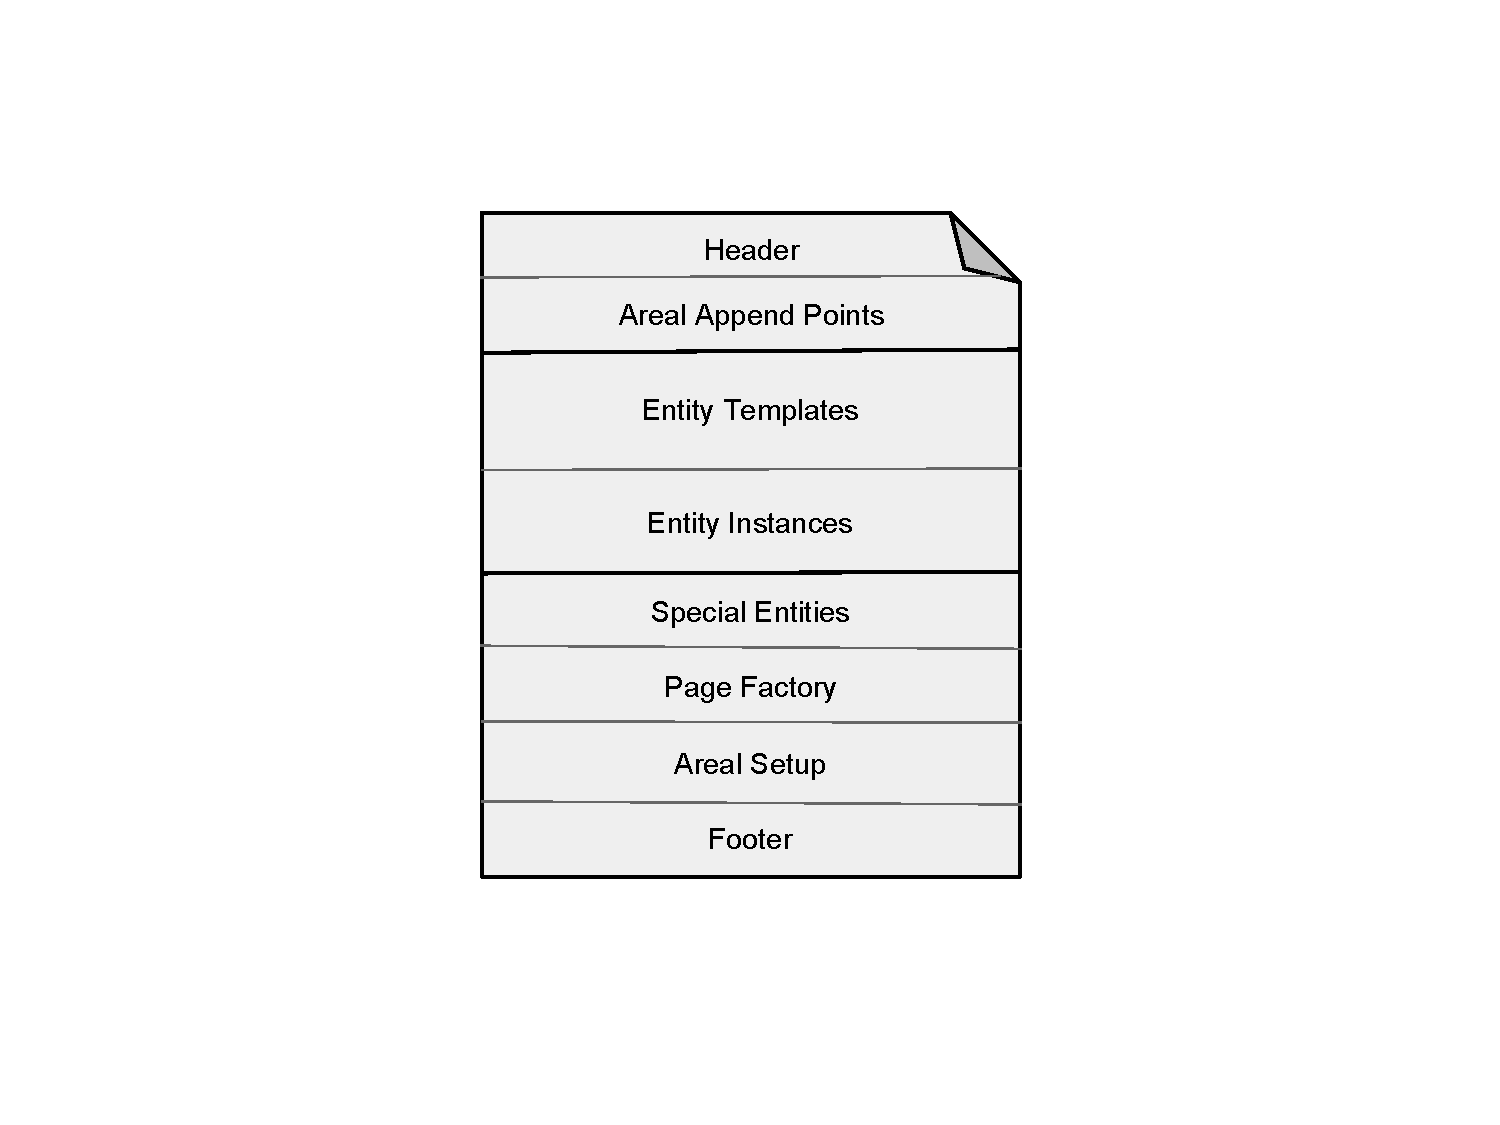
\includegraphics[width=0.45\textwidth]{figures/zielarchitektur_aufbau.pdf}
  \caption{Aufbau einer Datei der Zielarchitektur.}\label{fig-zielarchitektur_aufbau}
\end{figure}

\section{Scala DSL}\label{sec-scalaDSL}

Architektureller Aufbau der auf Scala basierenden internen DSL. Wie in
Kapitel \ref{sec-dsl} beschrieben, wird eine interne DSL in eine bereits
existierende Wirts-Programmiersprache eingebettet und bildet somit
eine mehr oder weniger gewöhn\-liche Software-Bibliothek. Im Idealfall ist
die \emph{API} dieser Bibliothek in ihrer Einsatzdomäne sehr ausdrucksstark.
Wie die API in diesem Fall gestaltet wird, ist in Kapitel
\ref{sec-grammatikGestaltung} näher beschrieben. In Kapitel
\ref{sec-api-resultat} ist ein Beispiel für ein lauffähiges
Dokumentenskript gegeben.

Wie der Generator bzw. Builder aufgebaut ist, wird in
Kapitel \ref{sec-generator} erklärt.

Die gesamten Spezifikationen bzw. Anforderungen sind in Kapitel
\ref{sec-dsl_anforderungen} aufgelistet.

Ein Muster, welches eine wichtige Rolle bei der Erstellung von Dokumenten
spielt, ist der Vorwärtsverweis, also gegenseitige Verweise von Entitäten,
wie Texten, Bildern, etc., aufeinander. Für dieses Muster gibt es in Scala
eine ziemlich elegante Lösung. Siehe dazu Kapitel \ref{sec-forwardreference}.

Das Repositorium mit dem gesamten Quellcode, sowie dem Testcode
und entsprechenden Versionen als ZIP-Archiv herunterladbar ist auf Github bereitgestellt.
Unter \url{https://github.com/themerius/ScalTeX-DSL} sind sämtliche
Quellcodes.

\subsection{Anforderungen}\label{sec-dsl_anforderungen}

Wie auch das Javascript-Framework (Kapitel \ref{sec-ziel_anforderungen})
wird auch die DSL bzw. Generator mittels behavior-driven development entwickelt.
Als Testframework kommt das ausgezeichnete
\emph{scalatest}-Testframework\footnote{
\url{http://www.scalatest.org}} zum Einsatz.

\paragraph{DocumentTemplateSpec}

\begin{itemize}
  \item A Entity
  \begin{itemize}
    \item should be a half abstract type to make concrete
    \item should contain a template id name
    \item knows an append point where it will appended to a page
    \item should have an unique id
    \item should generate a JSON suitable for the template snippet
    \item should be optional nameable via a \$ method
    \item should be able to set it's name as property to an areal-object
  \end{itemize}
  \item A Page 
  \begin{itemize}
    \item is a special form of an entity
    \item defines several append points, where entities are hooked in
    \item defines for every append point a type, templateVariable and maximum height
  \end{itemize}
  \item A Tray 
  \begin{itemize}
    \item should have a list buffer for type T, for extending companion objects
  \end{itemize}
  \item A Areal 
  \begin{itemize}
    \item The Entity binding ++ 
    \begin{itemize}
      \item binds the entity-method to corrosponding the entity-class
      \item should register the entity implicit to the calling areal's companion object's list
      \item should be able to register the entities reference as property to the corrosponding areal
      \end{itemize}
    \item is related to an append point, where pages are appended to
    \item has as minimum one assigned default page
    \item extends ordinary scala objects
    \item should own a implicit reference onto itslef
    \item is able to change the page layout
    \item The Generator 
    \begin{itemize}
      \item produces out of the areal entity-list a json datastructure
      \item should accept a implicit reference onto a Builder
    \end{itemize}
  \end{itemize}
  \item A Builder 
  \begin{itemize}
    \item must have a companion object with a list of related areals, in the right predefined order
    \item should own a implicit reference onto itslef
    \item should set the areal append points in the right order
    \item should know all pages available for this template
    \item calls the Generator for every Areal to form the js entity instances
    \item should assemble the page factory
    \item should be able to manipulate document's name
    \item should assemble the configuration in js for the special entities like page header/footer
    \item should assemble the js areal setup code
    \item should generate the areal append points
    \item should have a `build` method for generating the document
    \item should have a `write` method to save the document as html
  \end{itemize}
  \item A TemplateStock
  \begin{itemize}
    \item should have a `headerTemplate` method with title argument
    \item getting all entity snippets as String with `entityTemplate` method
    \item should have a `footerTemplate` getter/setter
  \end{itemize}
\end{itemize}

\paragraph{LogicSpec}

\begin{itemize}
\item The Logic trait
\begin{itemize}
  \item is a abstract marker
\end{itemize}
\item A FigureNumber
\begin{itemize}
  \item should extend an entity with an figure number variable
  \item should count figures and set the appropriate number for the particular figure
\end{itemize}
\item A SectionNumber
\begin{itemize}
  \item should extend an entity with a section variable
  \item should extend an entity with a h variable
  \item A Chapter
  \begin{itemize}
    \item should count all chapters
  \end{itemize}
  \item A Section
  \begin{itemize}
    \item should count in it's capter all sections
  \end{itemize}
  \item A SubSection 
  \begin{itemize}
    \item should count in it's section all subsections
  \end{itemize}
  \item A SubSubSection
  \begin{itemize}
    \item should count in it's subsection all subsubsections
  \end{itemize}
  \item   A TableOfContents 
  \begin{itemize}
    \item should filter all instances of SectionNumber returned as List (pending)
    \item extends an areal class (pending)
  \end{itemize}
\end{itemize}
\item A PythonScript
\begin{itemize}
  \item should construct a py-file out of a string (pending)
  \item should be able to execute the py file and its catch the std:out (pending)
\end{itemize}
\end{itemize}

\subsection{API Design}\label{sec-api-design}

Wie in Kapitel \ref{sec-dsl} definiert, entspricht eine interne DSL einer sehr
ausdrucksstarken Softwarebibliothek---sprich eine Bibliothek
mit einer intuitiven API, welche die Abstraktionen
des Aktionsraumes besonders herausarbeitet.
In diesem Fall ist der Aktionsraum ein Textsatzsystem. Der Benutzer will
also mit seinem DSL-Skript ein Dokument herstellen, welches als Produkt die
Zeilarchitektur aus Kapitel \ref{sec-zielarchitektur} produziert.
Ein Dokument setzt sich aus folgenden Bestandteilen
zusammen, siehe Kapitel \ref{sec-aufbauDokumente}:

\begin{itemize}
  \item Areal,
  \item Seitenlayout,
  \item Entitäten.
\end{itemize}

Zudem gibt es verschiedene Templates die austauschbar sein können, sofern
sie zum selbigen Dokumententypus, wie z.B. akademische Dokumente, gehören.
Ein ausführliches und zusammenhängendes Beispiel für ein DSL-Skript
ist im Anhang \ref{sec-api-resultat} zu finden.

\paragraph{Entitäten hinzufügen.} Mit Befehlen wie in Listing
\ref{api-entity} gezeigt, können Entitäten hinzugefügt werden.
Zeile 1 kann man so verstehen: „plus Abschnitt-Entität Überschrift.“
Zeile 3 „plus Unterabschnitt-Entität Unterüberschrift.“
In Zeile 5--7 wird eine mehrzeilige Text-Entität hinzugefügt.
In Zeile 9--12 wird ein Bild mit einer Internetbildquelle und einer
Beschreibung hinzugefügt.

\begin{lstlisting}[label=api-entity,caption=Entitäten hinzufügen.]
++ § "Ueberschrift"

++ §§ "Unterueberschrift"

++ txt """
  Lorem ipsum ...
"""

++ figure (
  src="http://domain.tld/pic.png",
  desc="Beschreibung fuer das Bild."
)
\end{lstlisting}

Zudem können flexibel verschiedene Entitäten zur API bei Bedarf
hinzugefügt werden, dies wird in Listing \ref{scala-syntax} bereits gezeigt.

\paragraph{Areale.}

Entitäten müssen einem Areal zugeordnet werden---dazu
melden diese sich implizit beim Areal an---wo
sie schlussendlich gesetzt werden sollen, siehe
Listing \ref{api-areal}. Jedes Areal
hat ein voreingestelltes Seitenlayout, welches aber auch bei Bedarf
geändert werden kann.

Ein odinäres Scalaobjekt, welches vom gewünschten Areal dessen Eigenschaften
erbt, dient als Container. In diesem Fall handelt es sich um das
Areal \emph{Document}, also das Areal welches das Hauptdokument beherbergt.
Es können mehrere Objekte vom gleichen Areal erben, diese sind aber logisch
dem gleichen Areal zugeordnet---so kann der Dokumentenquellcode besser
strukturiert werden.

\begin{lstlisting}[label=api-areal,caption=Areale bilden.]
object MeinAreal extends Document {
  // Entitaeten koennen hier eingefuegt werden.
  // Aenderung des Seitenlayouts:
  change page_to pageInstance
  // weitere Entitaeten, auf neuem Seitenlayout.
  // Expliziter Seitenumbruch funktioniert mit:
  newpage
  // weitere Entitaeten; jetzt auf neuer Seite.
}
\end{lstlisting}

\paragraph{Referenzierungen.} Referenzierungen sind ein
integraler Bestandteil von Dokumenten,
mit einer erschwerenden Anforderung: Referenzierungen auf eine Entität kann
in einem Dokument schon \emph{vor} dessen eigentlichen Deklaration vorkommen.
Wie dieser Umstand mit einem Trick gelöst werden kann, ist in Kapitel
\ref{sec-forwardreference} aufgeführt.

In Listing \ref{api-refs} wird ein solcher Verweis im DSL-Skript gezeigt.
Man beachte das \$ am Stringliteral in Zeile 6, welches dem Stringliteral
die Fähigkeit gibt, Referenzierungen anzunehmen. Innerhalb des
Stringliterals in Zeile 9 steht die eigentliche, beginnend mit \$\{
und endend mit \}, Referenz zur Bildentität aus Zeile 13.
Die Bildentität wird mit einem \$ entsprechend benannt und
referenzierungsfähig gemacht, wobei auch eine \emph{gewöhnliche}
Scalavariable verwendet werden könnte, statt der \$-Notation.

\begin{lstlisting}[label=api-refs,caption=Referenzierungen im DSL-Skript.]
object MeinAreal extends Document {
  ++ § "Ueberschrift"

  ++ §§ "Unterueberschrift"

  ++ txt $"""
    Lorem ipsum ...
    Die Referenz auf Abbildung
    ${MeinAreal.bildname.figureNumber}.
    ... lorem ipsum.
  """

  ++ $ "bildname" figure (
    src="http://domain.tld/pic.png",
    desc="Beschreibung fuer das Bild."
  )
}
\end{lstlisting}

\paragraph{Dokument erstellen.} Zunächst müssen die Areale in der gewünschten
Reihenfolge instanziiert werden, dazu melden sie sich implizit beim
\emph{Builder} an, um insbesondere ihre Reihenfolge innerhalb des Dokuments zu
definieren; wie in Listing \ref{api-builder} dargestellt.
Danach werden die verschiedenen Arealobjekte
aufgerufen, was auch die Reihenfolge der Entitäten innerhalb des Dokuments
definiert.
Auch der Builder bedient sich wieder eines normales Scalaobjets als Container.

\begin{lstlisting}[label=api-builder,caption=Dokument erstellen.]
object MeinDokument extends FraunhoferReportBuilder {
  new Document  // das Hauptdokument-Areal.

  MeinAreal
  // weitere Areal-Container aufrufen

  def main(args: Array[String]) {  // Programmeinstiegspunkt.
    write("_output/output.html")   // Dokument als html speichern.
  }
}
\end{lstlisting}


\subsection{Generator}\label{sec-archi-generator}

Auf Abbildung \ref{fig-uml_generator} ist der architekturelle Aufbau
des Generators zu sehen. Wobei der \emph{TemplateStock (Mixin\footnote{
Eine „wiederverwendbare Sammlung von Methoden und Attributen.“
\url{http://de.wikipedia.org/wiki/Trait_(Programmierung)}.
})}
HTML-Snippets lagert, woraus sich der \emph{Builder} bedienen kann.
Der Builder kennt die im Dokument vorhandenen Areale und damit auch dessen
Entitäten. Der Builder produziert aus jeder Entität das HTML-Gegenstück
und ordnet sie dem entsprechenden Areal zu, wobei auch entsprechende
Areale auf der JavaScript-Seite vom Builder konfiguriert werden.
Kurz gesagt, der Builder stellt eine komplette HTML-Datei passend für die
Zielarchitektur her, wie in Kapitel \ref{sec-html-datei} erklärt.

\begin{figure}[h!]
  \centering
    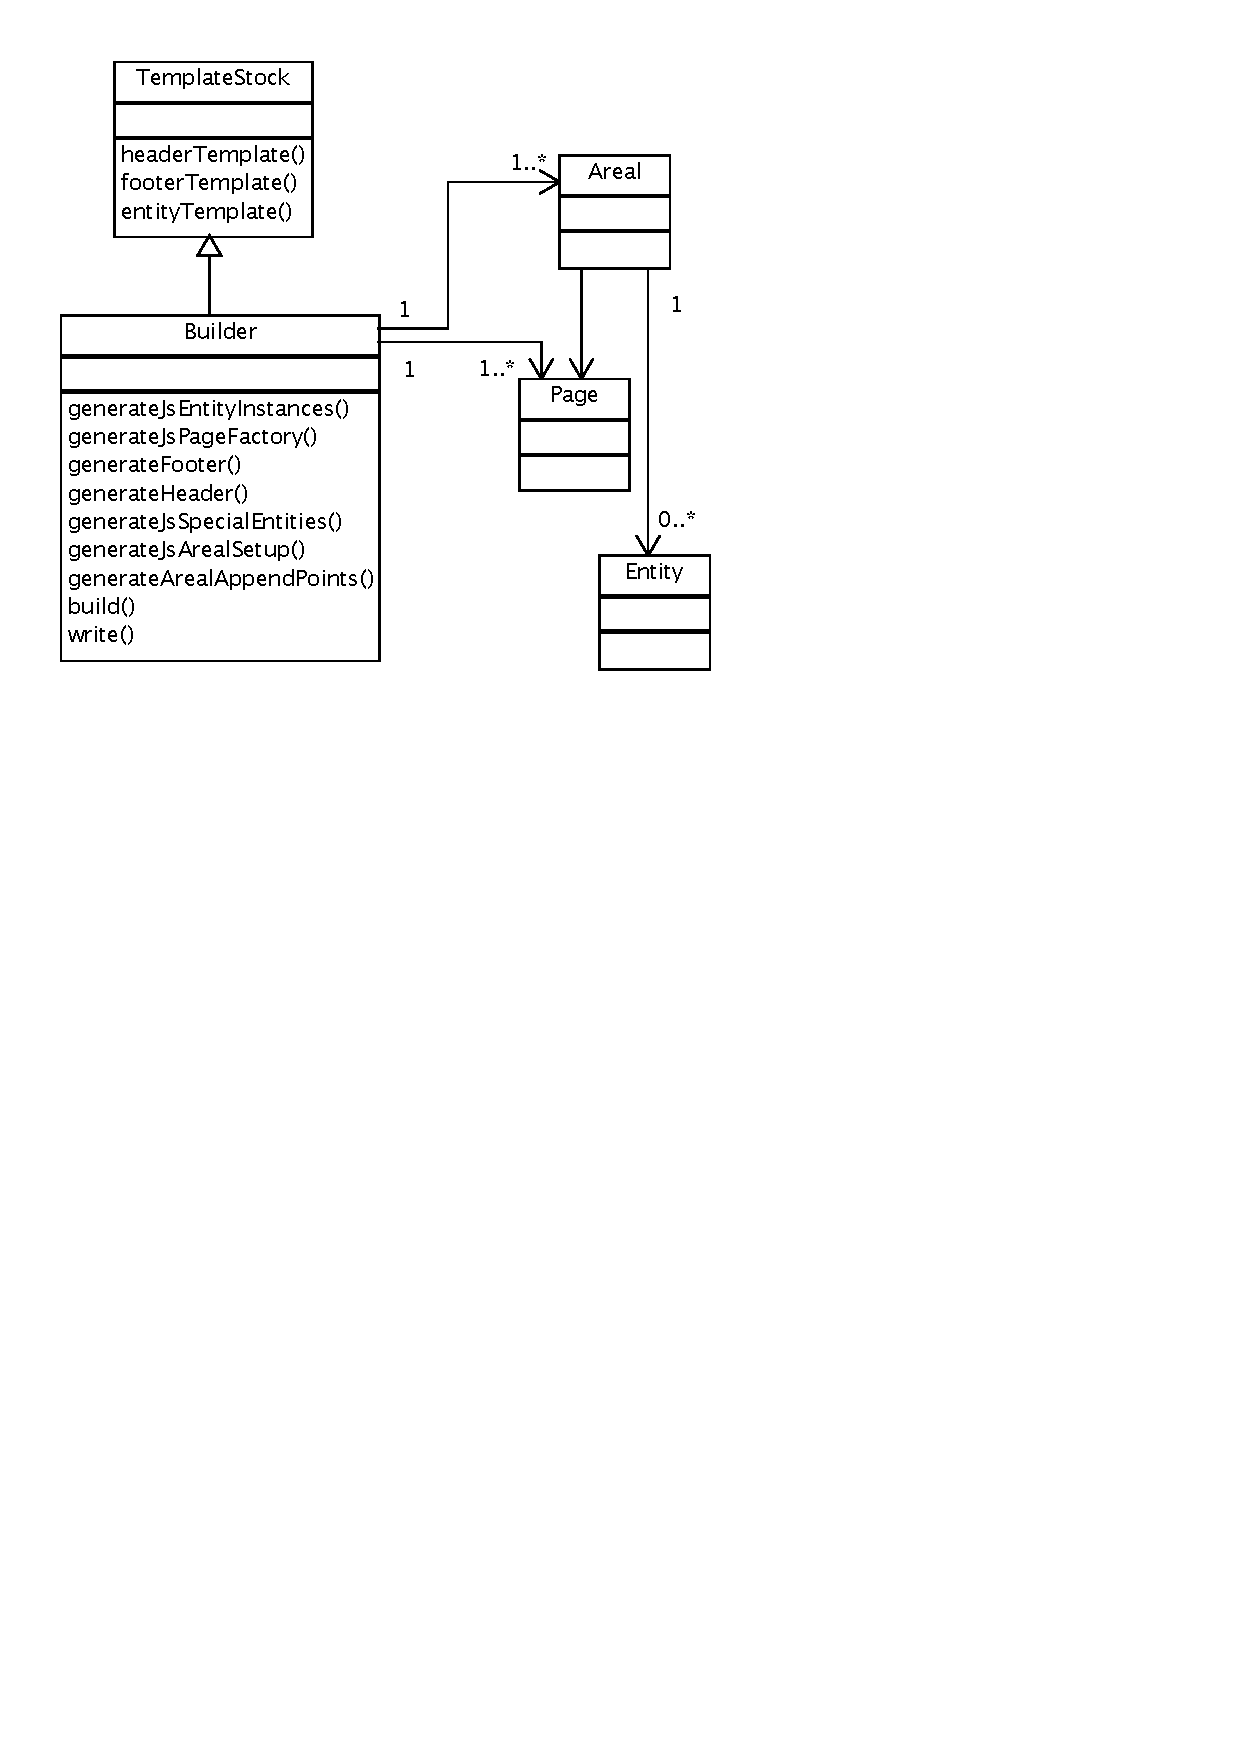
\includegraphics[width=0.6\textwidth]{figures/uml_generator.pdf}
  \caption{Aufbau des Generators des Anwendungsfalls in Scala.}\label{fig-uml_generator}
\end{figure}


\subsection{Vorwärtsverweis Muster}\label{sec-forwardreference}

Das Problem des
Vorwärtsverweises\footnote{Engl. \emph{forward reference}} tritt auf,
wenn z.B. in einem Text auf eine Abbildung
verweisen wird, welche innerhalb des Programmflusses aber erst später verfügbar
wird. Beispiel:

\begin{lstlisting}
... auf Abbildung {Reference} ist zu sehen ...

Reference = new Figure(...)
\end{lstlisting}

Hier wird also auf \verb|Reference| bereits zugegriffen,
bevor sie überhaupt existiert. Erschwerend kommt hinzu, dass die
Reihenfolge der Entitäten (Texte, Bilder, etc.) nicht verändert werden darf.
Die Abbildung soll also an der Position im Dokument erscheinen, an der sie
auch im Dokument-Quellcode geschrieben wurde, da es sich hier um eine DSL
handelt, die sich möglichst nahe am eigentlichen Dokument orientiert.

\subsubsection{Closure}\label{sec-closure}

Insbesondere funktionale Programmiersprachen wie Scala haben die
Möglichkeit Closures (\cite{scala-ref} Kapitel 6.23) zu bilden,
d.h. Teile des Geltungsbereichs (Scope)
der äußeren Funktion kann von der inneren Funktion beibehalten werden,
auch wenn der Geltungsbereich der äußeren Funktion bereits verwirkt ist.

\begin{lstlisting}
def outer_func = {
  val v = 15
  (x: Int) => x + v  // lambda function
}
\end{lstlisting}

Auf \verb|v| kann noch über die Lambda-Funktion zugegriffen werden,
selbst wenn \verb|outer_func| nicht mehr existiert. Teile des
\verb|outer_func|-Geltungsbereiches werden quasi mitgezogen.

Genau mit dieser Technik kann man den Vorwärtsverweis in den Griff bekommen.
Es wird der äußere Geltungsbereich eines Objekts nach innen gezogen,
um dort später, wenn alle Entitäten bekannt sind und die Referenz aufgelöst
wurde, darauf zuzugreifen.

\begin{lstlisting}
object O {
  val text = () => s"… auf Abbildung $reference ist zu sehen …"
  val reference = 3
}

O.text()  // wenn reference vorhanden
\end{lstlisting}

Hier wird zudem die Eigenschaft des \verb|object| ausgenutzt,
dass die im \verb|object| genannten Variablen immer schon vom Compiler
zumindest mit einer \verb|null|-Referenz exisieren, aber die Reihenfolge
der eigentlichen Instanziierung nicht verändert wird. Durch das
\verb|lazy|-Keyword von Scala, würde die Reihenfolge modifiziert werden
und ist dadurch nicht praktikabel.

Nachteil hier ist, dass der Domänen-Benutzer innerhalb der DSL diese
\verb|() => s""| Magie schreiben müsste---was zu Verwirrung und
Unverständnis führen würde.


\paragraph{Verbesserung für den Domänen-Benutzer}

Ideal wäre also nun eine Lösung inder der Domänen-Benutzer keine
Aufmerksamkeit auf die Closure-Magie verschwenden muss.

In Listing \ref{stringcontext} wird auf den ab Scala 2.10 verfügbaren
\verb|StringContext| (\verb|s"…"|)
gesetzt. \cite{scala-stringInterpolation}
Dieser lässt sich so erweitern, dass
sich die Closure-Magie verstecken\footnote{Entstammt meinen
Stackoverflow-Fragen: \url{http://stackoverflow.com/questions/13307418} und
\url{http://stackoverflow.com/questions/13270906}.} lässt und somit in die API
gezogen wird und der Domänen-Benutzer davon gar nichts mitbekommt.

\begin{lstlisting}[label=stringcontext,caption=Erweiterter StringContext]
implicit def byname_to_noarg[A](a: => A) = () => a

case class StringContext(parts: String*) {
  def $ (args: (() => Any)*) = () => {
    val unpacked_args = args.map(a => a())
    scala.StringContext(parts: _*).s(unpacked_args: _*)
  }
}

object O {
  val text = $"… auf Abbildung $reference ist zu sehen …"
  val reference = 3
}

O.text()  // wenn reference vorhanden
\end{lstlisting}

\verb|byname_to_noarg| ist eine implizite Konvertierung von einem
beliebigen Typ \verb|A| mit Call-by-Name\footnote{Ein Call-by-Name
Parameter wird bei jedem Funktionsaufruf erneut evaluiert.
(\cite{scala-ref} Kapitel 4.6.1)}
\verb|a: => A| in eine Lambda-Funktion \verb|() => a|.

\verb|def $| fügt die Möglichkeit hinzu \verb|$"…"| als individuell
angepassten \verb|StringContext| zu verwenden. Es wird eine variable 
Argumentenliste mit den implizit zu Call-by-Name konvertierten Argumenten
aus einem beliebigen \verb|$"…"|-String übergeben und in ein Closure gepackt,
welches erst dann ausgeführt wird, wenn die Referenzen auch tatsächlich
vorhanden sind.


\section{Ergebnis}

\paragraph{Zielarchitektur.}
In Kapitel \ref{sec-zielarchitektur} ist ein JavaScript-Framework entstanden,
welches die Darstellung eines „klassischen“ Dokuments mit Webtechnologie
ermöglicht.
Es gliedert ein Dokument in seine Areale, Seitenlayouts und Entitäten auf
und stellt diese als entsprechende Templates bereit, so dass die DSL sich
nicht um die Darstellung kömmern muss, sondern lediglich das
JavaScript-Framework konfigurieren muss.
Jedoch wohl das wichtigste Merkmal ist die Fähigkeit ein Webdokument wie
ein Printdokument aussehen zu lassen.

Im Zuge der Entwicklung des JavaScript-Frameworks sind zwei Dokumententemplates
entstanden:

\begin{enumerate}
  \item Der \emph{Fraunhofer Bericht} basierend auf dem
        Fraunhofer Corporate Design,
  \item Adaption der \emph{EPO Patentschrift} des europäischen Patentregisters.
\end{enumerate}

Es konnte jedoch nicht alles umgesetzt werden, z.B. insbesondere fehlt
der Zielarchitektur noch die Unterstützung für Fußnoten, aber auch die
Fähigkeit übergroße Entitäten auf mehere Seiten aufzuteilen. Natürlich gibt
es noch wesentlich mehr Dinge die umgesetzt werden könnten, um über den Status
eines Prototypes hinauszugehen.

\paragraph{DSL und Logik.}
Die DSL mit der Generatorlogik ist in Kapitel \ref{sec-scalaDSL} erklärt.
Die interne Scala-DSL gibt dem Benutzer ein intuitives Werkzeug zur Hand,
mit dessen Hilfe er ein textuelles Dokumentenerstellungsskript erstellen kann,
ohne wirklich zu merken, dass er eigentlich reinen Scala-Code schreibt.
Durch diverse Abstraktionen die mit Scala ermöglicht werden, gelingt es
sehr viele Implementierungsdetails in tiefere Ebenen zu verstecken, so
dass ein neues Template sogar von einem DSL-Benutzer, mit einer kurzen
Anleitung, seblst erstellt oder ein vorhandenes erweitert werden kann.
Schlussendlich generiert die DSL eine HTML-Datei die das in der DSL
beschriebene Dokument enthält, die das o.g. JavaScript-Framework verwendet.
Ein Webbrowser der die HTML-Datei öffnet, setzt\footnote{
Ein Begriff aus dem Handwerk des Buchdrucks.
\url{http://de.wikipedia.org/wiki/Schriftsetzer}.}
dann mithilfe des JavaScript-Frameworks das Dokument.

Ähnlich ist es auch bei der DSL, dort wurden auch nur die wichtigsten Funktionen
implementiert, um zu zeigen, dass die Umsetzung in einem überschaubaren
Rahmen möglich ist.

\subsection{Kleine Statistik}

Die Zielarchitektur hat leicht über 300 Zeilen JavaScript-Code und
fast 500 Zeilen Testcode. (Ohne HTML/CSS der Templates.)

Die DSL und Logik haben knapp 400 Zeilen Scala-Code und leicht über 700 Zeilen
Testcode. Wobei ein Template, wie der Fraunhofer Bericht, alleine nochmals
ca. 350 Zeilen Code umfasst, jedoch sind davon ca. 100 Zeilen HTML-Template-Code
der Zielarchitektur. (Ohne DSL-Skript Beispiele.)
